\section{Figuras}

Las \textbf{figuras} son muy similares a las imágenes en \LaTeX, solo que este requiere de los comandos \textbf{\textbackslash{begin}} y \textbf{\textbackslash{end}}, seguido de \textbf{\{figure\}} para indicar una figura, los corchetes de ubicación [] también hacen aparición aquí, se requiere el paquete \textbf{graphicx}, importar las imágenes a esta plataforma para así adjuntarlas al documento.

Al igual que las imágenes, se adjuntan utilizando el comando \textbf{\textbackslash{includegraphics\{\}[]}}, que de igual forma, tiene el parámetro del tamaño entre corchetes y la figura propiamente dentro de llaves, la cual debe haber sido importada a esta plataforma previamente. La \textit{Figura \ref{fig: 4}} es el ejemplo de una imagen contenida por una figura:
\begin{lstlisting}
    \begin{figure}[H]
        \begin{center}
            \includegraphics [width=10cm]{ejemplo_latex.png}
        \end{center}
    \end{figure}
\end{lstlisting}
\begin{figure}[H]
    \begin{center}
        \caption{Figura de ejemplo}
        \label{fig: 4}
        \includegraphics[width=10cm]{recursos/ejemplo_latex.png}
    \end{center}
\end{figure}

\textit{Nota}: se recomienda trabajar las imágenes como figuras, ya que este contenedor permite asignarle nombres y etiquetas a las imágenes, como se ve en el ejemplo anterior.



\section{Comandos personalizados}

El comando \textbf{\textbackslash{newcommand}} nos permite tomar otros comandos y crear uno nuevo o uno personalizados, de tal forma que nos ahorre algo de tiempo, escritura y código.


\subsection{Sin parámetros}

Supongamos que queremos un acceso más rápido para el comando \textbf{\textbackslash{mathbb}} (previamente debimos haber agregado el paquete \textbf{amsfonts} para que este comando pudiera servir), para escribir el símbolo de los números reales, utilizamos \textit{newcommand\{\}\{\}}, en el primer par de llaves se escribe \textbf{\textbackslash}, seguido por el nombre que le darás a este nuevo comando, y en las segundas llaves, escribimos el comando que se ejecutará cuando llames al comando que apenas se está creando; no olvide que la creación de nuevos comandos puede ser antes o después al comienzo del documento:
\begin{lstlisting}
    \usepackage{asmfonts}
    
    \newcommand{\R}{\mathbb{R}}
    
    \begin{document}
        \R
    \end{document}
\end{lstlisting}

\newcommand{\R}{\mathbb{R}}

El resultado de usar nuestro nuevo comando creado \textbf{\textbackslash{R}} es: los números reales son $\R$


\subsection{Con parámetros}

Podemos crear comandos nuevos que involucren la entrada de datos para que estos desplieguen algún texto o resultado. En este caso buscamos crear un comando que reciba dos números o letras para formar un vector, involucraremos la creación de una matriz durante el camino, para ello, utilizamos el comando \textbf{newcommand\{\}[]\{\}}, el primero y último es lo mismo que el anterior ejemplo, el segundo parámetro se encuentra entre corchetes, y en este se definirán el número de parámetros para el nuevo comando (si son tres parámetros, para pasárselos al comando que se ejecutará cuando llamemos al que estamos creando actualmente, debemos poner el símbolo \#, seguido del número de parámetro que deseemos: \#1, \#2, \#3, ..., \#n):
\begin{lstlisting}
    \begin{document}
        \newcommand{\M}[2]{
            \begin{bmatrix}
	            #1\\
	            #2\\
            \end{bmatrix}
        }
    \end{document}
\end{lstlisting}
\newcommand{\M}[2]{\begin{bmatrix}
	#1\\
	#2\\
\end{bmatrix}
}

Primer intento, le pasamos a \textbf{\textbackslash{M\{\}\{\}}} los valores 1 y 2, el resultado es: $\M{1}{2}$

Segundo intento, le pasamos a \textbf{\textbackslash{M\{\}\{\}}} los valores a y b, el resultado es: $\M{a}{b}$
